%!TEX root = main.tex

The $\extract$, $\replace$ and $\replaceall$ functions can be accurately modeled using PSSTs.
That is, we can reduce satisfiability of our string logic to satisfiability of a logic containing only concatenation, PSST transductions, and membership of regular languages.

\begin{lemma}\label{lem-str-fun-to-psst}
    The satisfiability of $\strline$ reduces to the satisfiability of boolean combinations of formulas of the form $z=x \concat y$, $y=\cT(x)$, and $x \in \cA$, where $\cT$ is a PSST and $\cA$ is an FA.
\end{lemma}

First, observe that regular constraints (aka membership queries) $x \in e$ can be reduced to FA membership queries $x \in \cA$ using standard techniques.
Features such a greediness and capture groups do not affect whether a word matches a {\regexp}, they only affect \emph{how} a string matches it.
Thus, for  regular constraints, these features can be ignored and a standard translation from regular expressions to finite automata can be used.

The $\extract_{i,e}$ function can function be defined by a PSST $\cT_{i,e}$ obtained from the PSST $\cT_e$ (see Section~\ref{sect:regextopsst}) by removing all the string variables, except the string variable $x_{e'}$, where $e'$ is the subexpression of $e$ corresponding to the $i$th capturing group, and setting the output expression of the final states as $x_{e'}$.
%First, observe that membership tests $x \in e$ can be reduced to FA membership tests $x \in \cA$ using standard techniques.
%Features such a greediness and capturing groups do not affect whether a word matches a regular expression, they only affect \emph{how} a word matches a expression.
%Thus, for membership tests, these features can be ignored and a standard translation from regular expressions to finite automata can be used.

We give a sketch of the encoding of $\replaceall$ here.
Full formal details are given in Appendix~\ref{appendix:sec-extract-replace-to-psst}.
The encoding of $\replace$ is almost identical to that of $\replaceall$.

A call $\replaceall_{\pat, \rep}(x)$ replaces every match of $\pat$ in the value of $x$ by a value determined by the replacement string $\rep$.
In addition to literal characters, $\rep$ may also contain references $\$i$, $\refbefore$, or $\refafter$.
The first step in our reduction to PSSTs is to eliminate the special references $\$0$, $\refbefore$, and $\refafter$.
In essence, this simplification uses PSST transductions to insert the contextual information needed by $\refbefore$ and $\refafter$ alongside each substring that will be replaced.
Then, the call to $\replaceall$ can be rewritten to include this information in the match, and use standard references ($\$i$) in the replacement string.
The reference $\$0$ can be eliminated by wrapping each pattern with an explicit capturing group.

We show informally how to construct the PSST for $\replaceall_{\pat, \rep}$ where all the references in $\rep$ are of the form $\$i$ with $i > 0$.
The full reduction is given in the appendix.

Let $\rep = w_1 \$i_1 w_2 \cdots w_k \$i_k w_{k+1}$. Moreover, let $e'_{i_1},\ldots, e'_{i_k}$ be the subexpressions of $\pat$ corresponding to the $i_1$th, $\ldots$, $i_k$th capturing groups.
Note, in particular, that we may have $i_j = i_{j'}$ with $j \neq j'$.

By abuse of notation, we will write
$\rep[x_{e'_{i_1}}/\$i_1,\cdots,x_{e'_{i_k}}/\$i_k]$
to denote the replacement of the references, in order of appearance, by the contents of the variables $x_{e'_{i_j}}$.
For example, if
$\rep = a \$1 a \$2 a \$1 a$
then
$\rep[x_{e'_{i_1}}/\$i_1, x_{e'_{i_2}}/\$i_2,x_{e'_{i_3}}/\$i_3]$
is $a w_1 a w_2 a w_3 a$ when $w_j$ is the value stored in $x_{e'_{i_j}}$.

Although, in this notation, it is possible to substitute different occurrences of a reference with different word values, our encoding will always substitute the same value.
That is, if $i_j = i_{j'}$ then $x_j$ will contain the same value as $x_{j'}$.
We use two variables in this case to satisfy the copyless property~\cite{AC10}, which leads to improved complexity results in some cases (discussed in the sequel).
If we tried to use a single variable – e.g. $\rep[x/\$i_1,x/\$i_2]$ – then the resulting transition in the encoding below would not be copyless.

 Suppose $\cT_\pat = (Q_{\pat}, \Sigma, X_{\pat}, \delta_{\pat}, \tau_{\pat}, q_{\pat,0}, (F_{\pat,1}, F_{\pat,2}))$.
Then $\cT_{\replaceall_{\pat,\rep}}$ is obtained from $\cT_\pat$ by adding a fresh state $q'_0$ such that (see Fig.~\ref{fig-psst-replaceall})
\begin{itemize}
    \item $\cT_{\replaceall_{\pat,\rep}}$ goes from $q'_0$ to $q_{\pat,0}$ via an $\varepsilon$-transition of higher priority than the non-$\varepsilon$-transitions, in order to search the first match of $\pat$ starting from the current position,
        %
    \item when $\cT_{\replaceall_{\pat,\rep}}$ stays at $q'_0$, it keeps appending the current letter to the end of $x_0$, which stores the output of $\cT_{\replaceall_{\pat,\rep}}$,
        %
    \item starting from $q_{\pat, 0}$, $\cT_{\replaceall_{\pat,\rep}}$ simulates $\cT_\pat$ and stores the matches of capturing groups of $\pat$ into the string variables, in particular,
    the matches of the $i_1$th, $\ldots$, $i_k$th capturing groups into the string variables $x_{e'_{i_1}}, \cdots, x_{e'_{i_k}}$ respectively,
        %
    \item when the first match of $\pat$ is found, $\cT_{\replaceall_{\pat,\rep}}$ goes from $f_{\pat,1} \in F_{\pat, 1}$ or $f_{\pat, 2} \in F_{\pat, 2}$ to $q'_0$ via an $\varepsilon$-transition, appends the replacement string, which is $\rep[x_{e'_{i_1}}/\$_{i_1}, \cdots, x_{e'_{i_k}}/\$_{i_k}]$, to the end of $x_0$, resets the values of al the string variables, except $x_0$, to $\nullchar$, and keeps searching for the next match of $\pat$.
\end{itemize}

It may be observed that the PSST will be copyless.
That is, the value of a variable is not copied to two or more variables during a transition.
In all but the last case, variables are only copied to themselves, via assignments of the form $x_{e'} = x_{e'} a$, $x_{e'} = x_{e'}$, $x_{e'} = \varepsilon$, or $x_{e'} = \nullchar$.
In the final case, when a replacement is made, the assignments are of the form
$x_0 = x_0 w_1 x_{e'_{i_1}} w_2 \cdots w_k x_{e'_{i_k}} w_{k+1}$
and
$x_{e'} = \nullchar$ for all the variables $x_{e'} \in X_\pat$.
Again, only one copy of the value of each variable is retained to the next step.

Copyful PSSTs are only needed when removing $\refbefore$ and $\refafter$ from the replacement strings.
To see this, consider the prefix preceding the first replacement in a string.
If $\refbefore$ appears in the replacement string, this prefix will be copied an unbounded number of times (once for each matched and replaced substring).
Conversely, references of the form $\$i$ are ``local'' to a single match.
By having a separate variable for each occurence of $\$i$ in the replacement string, we can avoid having to make copies of the values of the variables.

\begin{figure}[ht]
	\vspace{-2mm}
    \centering
    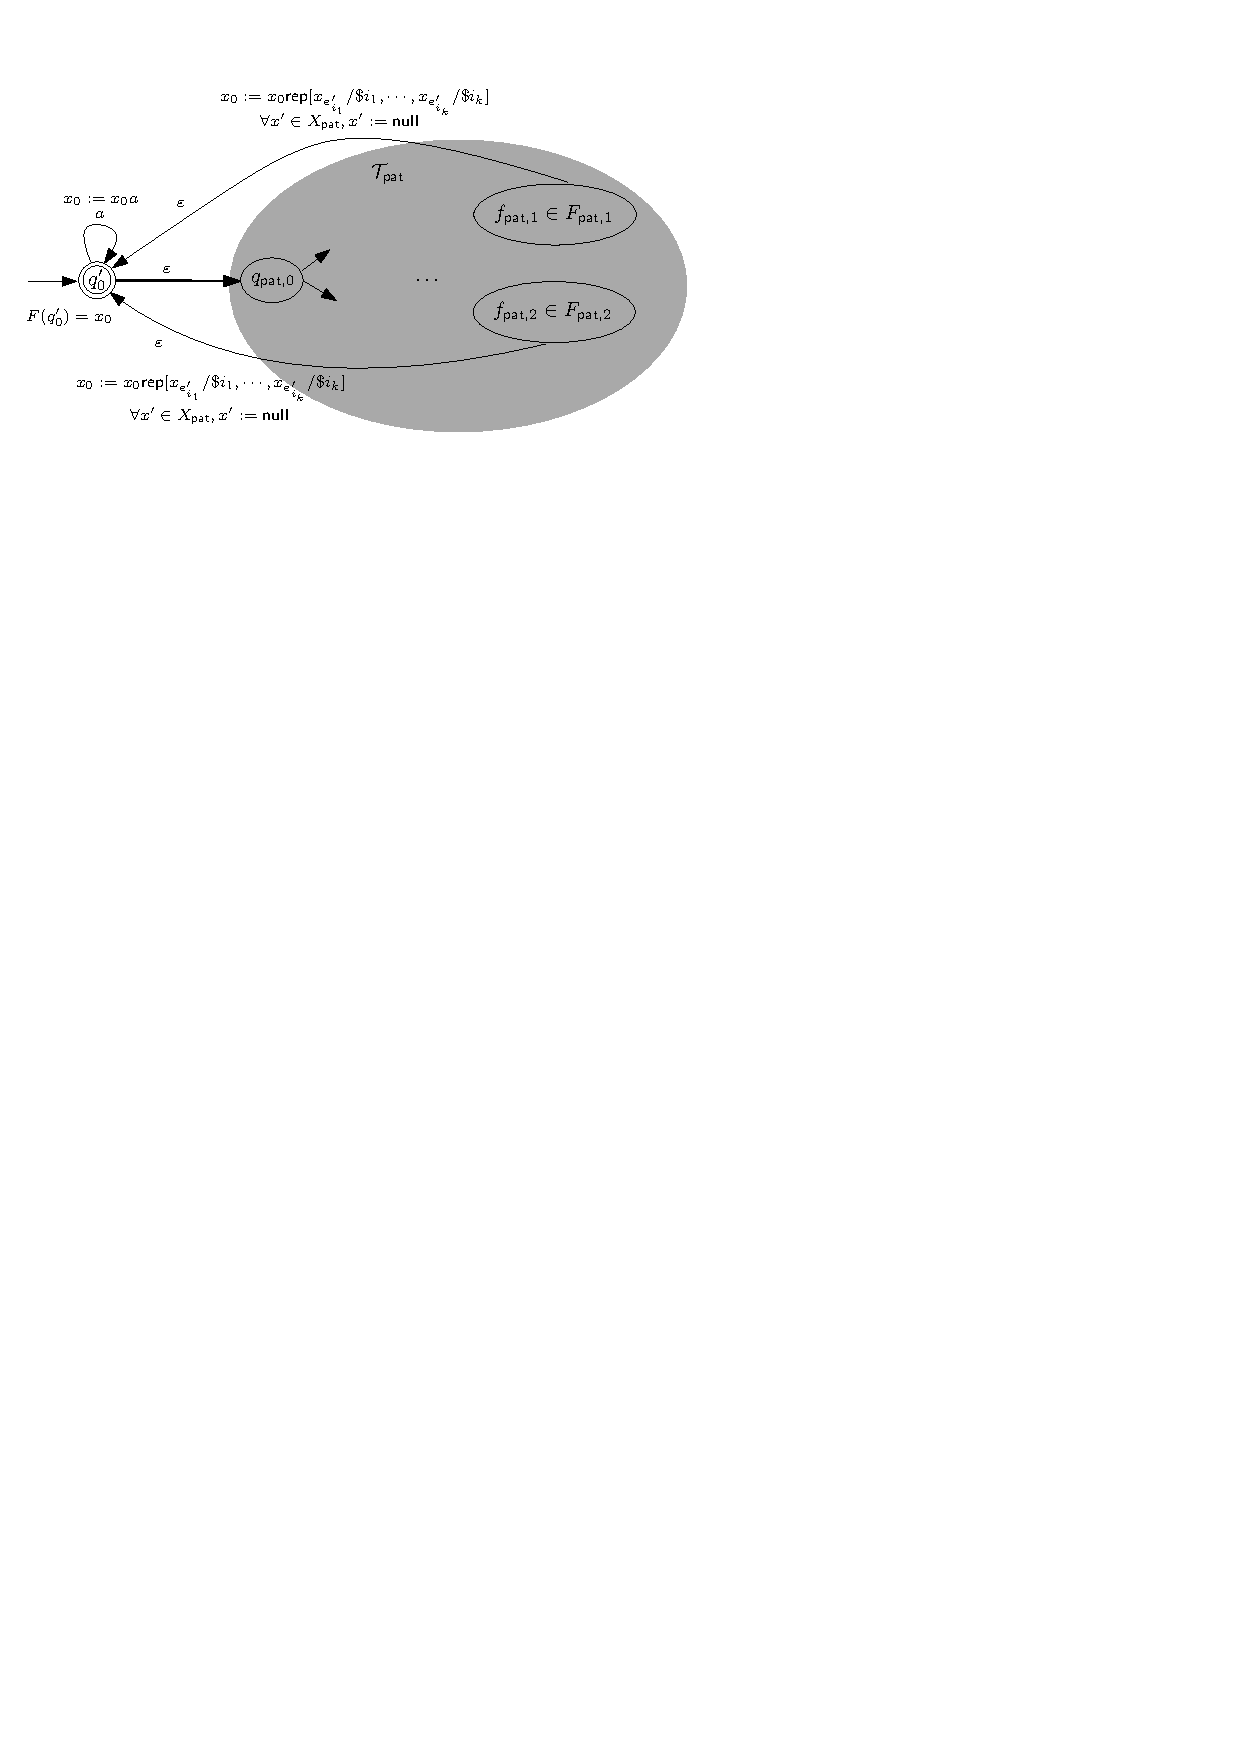
\includegraphics[scale=0.7]{psst-replaceall.pdf}
    \caption{The PSST $\cT_{\replaceall_{\pat,\rep}}$}
    \label{fig-psst-replaceall}
    \vspace{-2mm}
\end{figure}


